\chapter{Data Understanding}

\section{Initial Data Collection Report}

\paragraph{Data Requirements Planning}
The business objective is the development of a solution for the automatic aggregation of documents based on their topics. To achieve this goal, a sufficient number of documents are required. Also, the documents must contain enough text to be assigned a topic. After clustering the value of each expense in a cluster have to be summed, to gain the desired insight of spendings in one category. So the value an expense amounts to has to be included in the data.

\paragraph{Selection Criteria}
An initial look a the data has shown that each invoice item can easily contain more than 100 pieces of information, which can be considered as attributed in the dataset. The part of the data that is of interest for the research is the description and payment data. Other data needs to be retained for a coherent and informative presentation of the results, such as location information and information on seller and buyer.

\paragraph{Insertion of Data}
The insertion of data is concerned with the theoretical utilization of the data and problems arising during this process. The encoding and grouping of free text items is referenced as one concern in the \ac{CRISP-DM} user guide \cite[p.~38]{CRISPDM2000}. In this research the focus is on free text items, therefore this step will be discussed in detail in the following chapter. 
Other concerns are missing attributes. The dataset has already undergone a surface-level evaluation, which concludes that all relevant attributes are contained.

\section{Data Description Report}
The data is available as a local folder of size 5.12 GB, it contains 152,591 \ac{JSON} files. Each file represents one invoice document. The files are between 11 and 540 KB in size.

Each invoice contains specific header data, the detailed list of the 172 header fields is contained in the appendix \ref{invoice-header}. 

The items listed in one invoice are line items. The information about line items is contained in 32 features, also detailed in the appendix \ref{invoice-lines}.

\section{Data Exploration Report}

The target for aggregation being the descriptions of line items, this feature is explored first.

\paragraph{Descriptions}
The descriptions of invoice items vary greatly in their length. While the largest portion of descriptions is under 600 characters, there are outliers with over 1000 characters. 
\begin{figure}[ht]
	\centering
	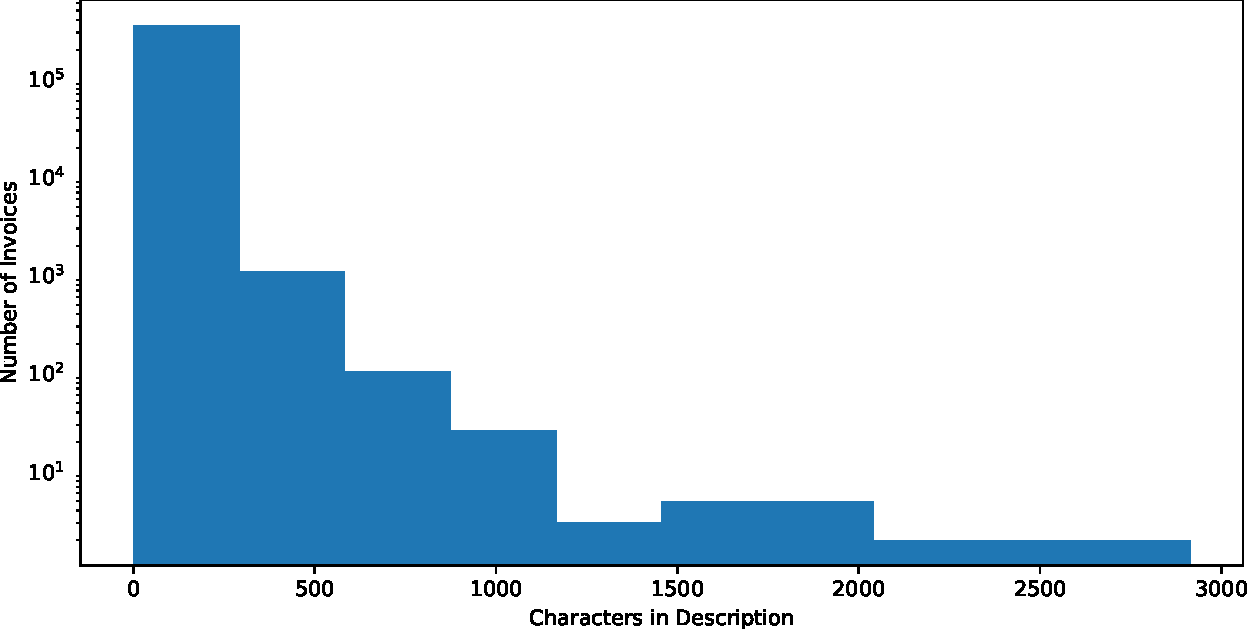
\includegraphics[height=8cm]{Bilder/hist_description.pdf}
	\caption{Histogram of Description Length}
	\label{fig:languages-bar}
\end{figure}

\paragraph{Language Distribution}
The description of the invoices is related to the feature 'language', which describes the language of the invoice and its text fields. The most popular languages are English, Spanish, and German. It is noticeable, that there are over 700 languages or combinations of more than one language. 58878 invoices were not assigned a language, which is roughly one third of the total number.
\begin{figure}[ht]
	\centering
	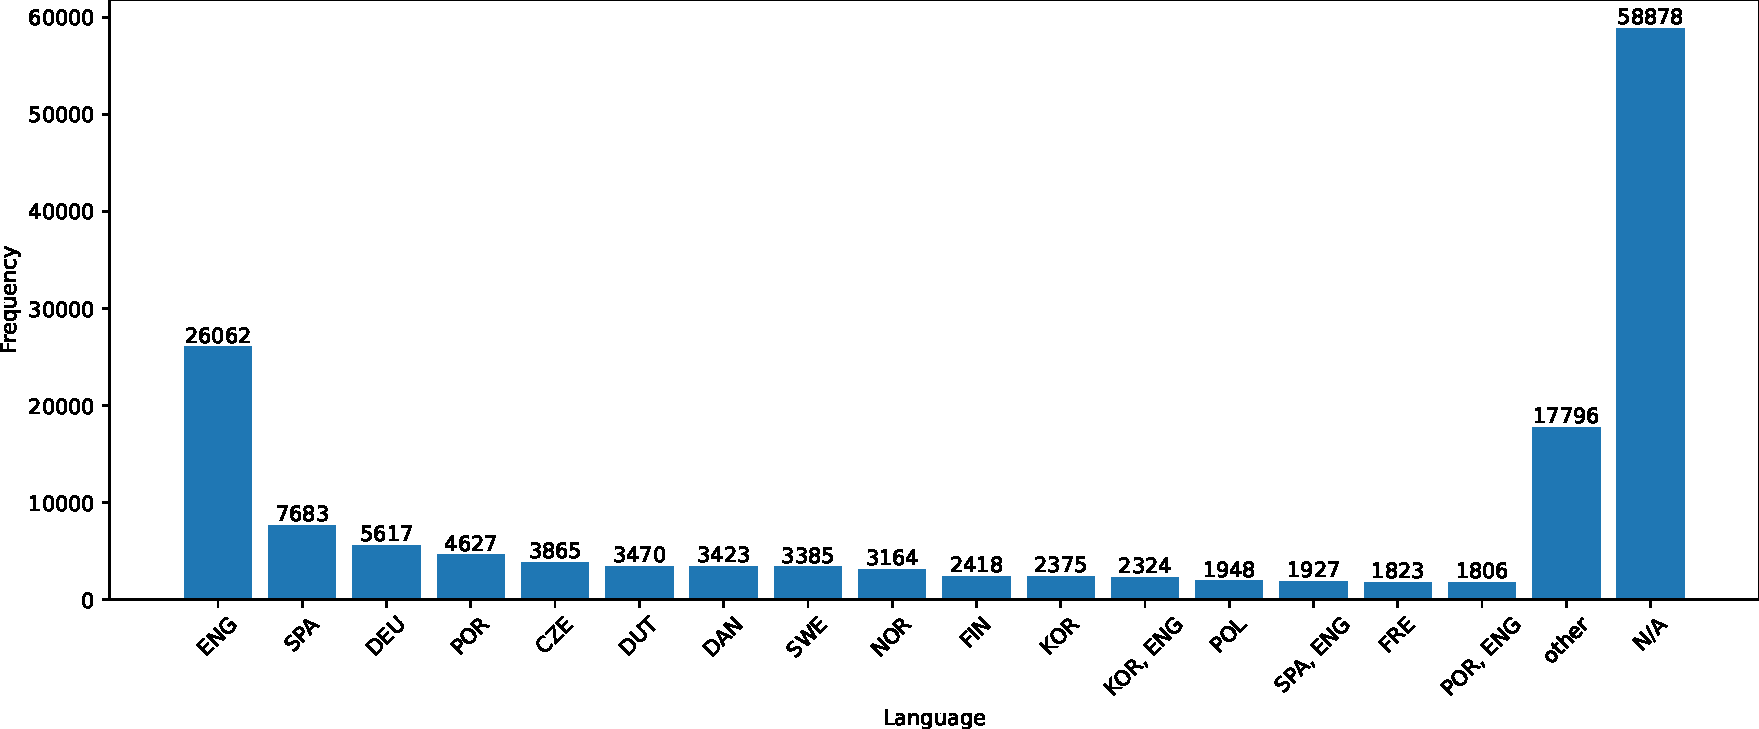
\includegraphics[height=6cm]{Bilder/languages.pdf}
	\caption{Number of Invoices per Language}
	\label{fig:languages-bar}
\end{figure}

For the cumulative distribution of the languages, N/A values were omitted. From the chart it can be inferred, that 80\% of invoices are in the top 16 languages. The slow rise after the top 80 languages indicates, that there are a lot of languages with a small number of invoices. This is also explained with a huge number of possible combinations of more than one language.
\begin{figure}[ht]
	\centering
	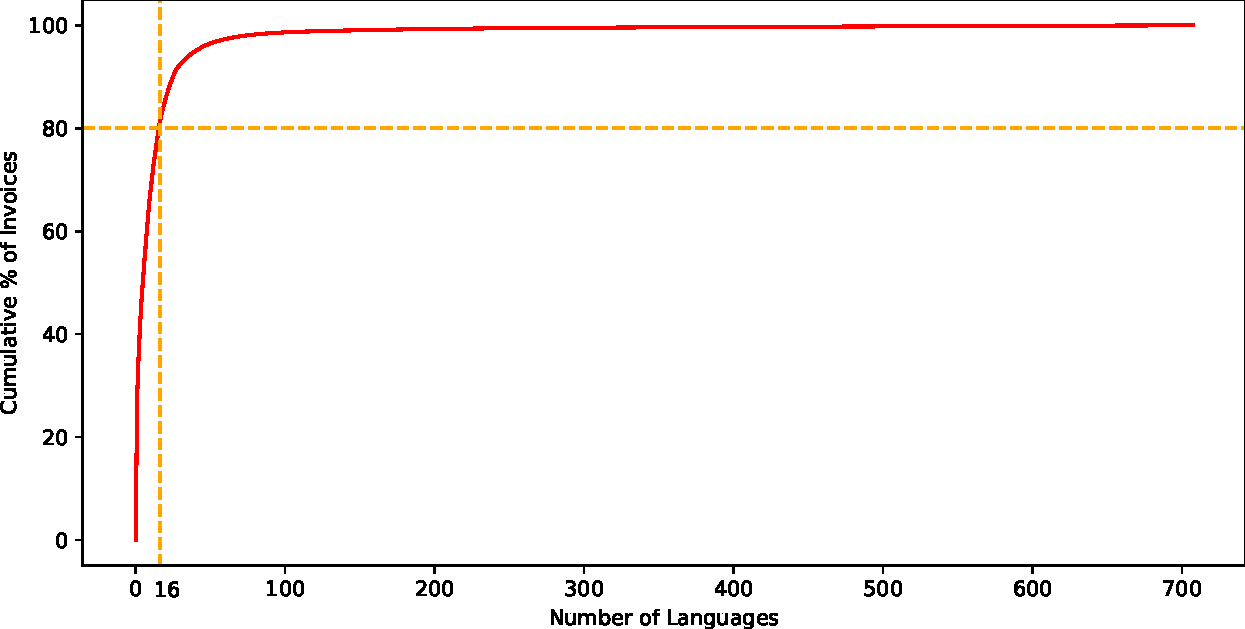
\includegraphics[height=6.5cm]{Bilder/languages_pareto.pdf}
	\caption{Percentage of Invoices by cumulative Number of Languages}
	\label{fig:languages-bar}
\end{figure}


\section{Data Quality Report}
DOes the data contain errors?
Are there missing values?
are all values plausible?
plot some stuff here
check number of fields in each record (?) maybe optional
